\chapter{Feature Matching and Outlier Rejection}\label{ch:matching}

The key idea of this work revolved around building 2D matches of points of which the 3D information was known. So in essence I built 3D matches using 2D methods.
\begin{figure}[ht]
    \centering
    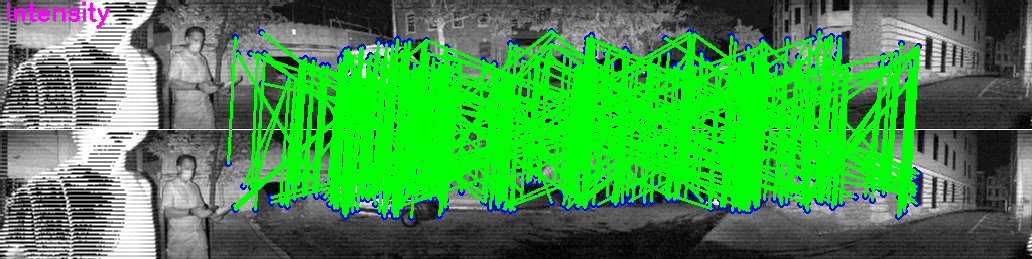
\includegraphics[scale = 0.34]{images/matching_+_outlier_rejection/orb_matches_unfiltered.png}
    \caption{Unfiltered ORB matches on intensity data}
    %label always in the end
    \label{fig:match_preview}
\end{figure}


Note that the upper half of \cref{fig:match_preview} is the current one while the lower part holds the previous stance with the detected points from the last extraction.

In order to compare the feature methods as well as the complementary data types the outlier rejection procedure has to be discussed.

\section{RANSAC Filtering}{
    The first filtering method performed was the well known non-deterministic RANSAC outlier Rejection. 
    Thanks to the projection based approach in this work a 2D – 2D RANSAC implementation could be applied.Concretely I made use of the RANSAC implementation in opencv's \textit{findHomography} method.

    \begin{figure}[ht]
        \centering
        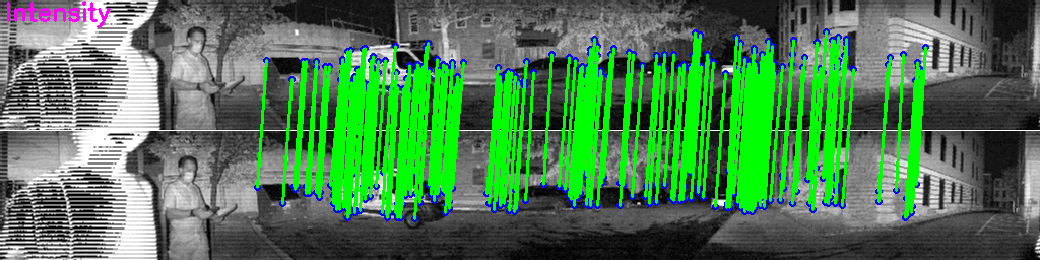
\includegraphics[scale=0.34]{images/matching_+_outlier_rejection/orb_matches_ransac_filtered.png}
        \caption{Ransac filtered}
        %label always in the end
        \label{fig:ransac_preview}
    \end{figure}
}

\section{Depth Problem}{
    The second match filtering performed accounted for depth inaccuracies for the matches considered. Just looking at the RANSAC filtered matches \cref{fig:ransac_preview} no flaw could really be detected. However as we are looking at 2D projections of 3D data we have to consider the depth as well. 

    \begin{figure}[ht]
        \centering
        \subfloat[RANSAC filtered matches]{
        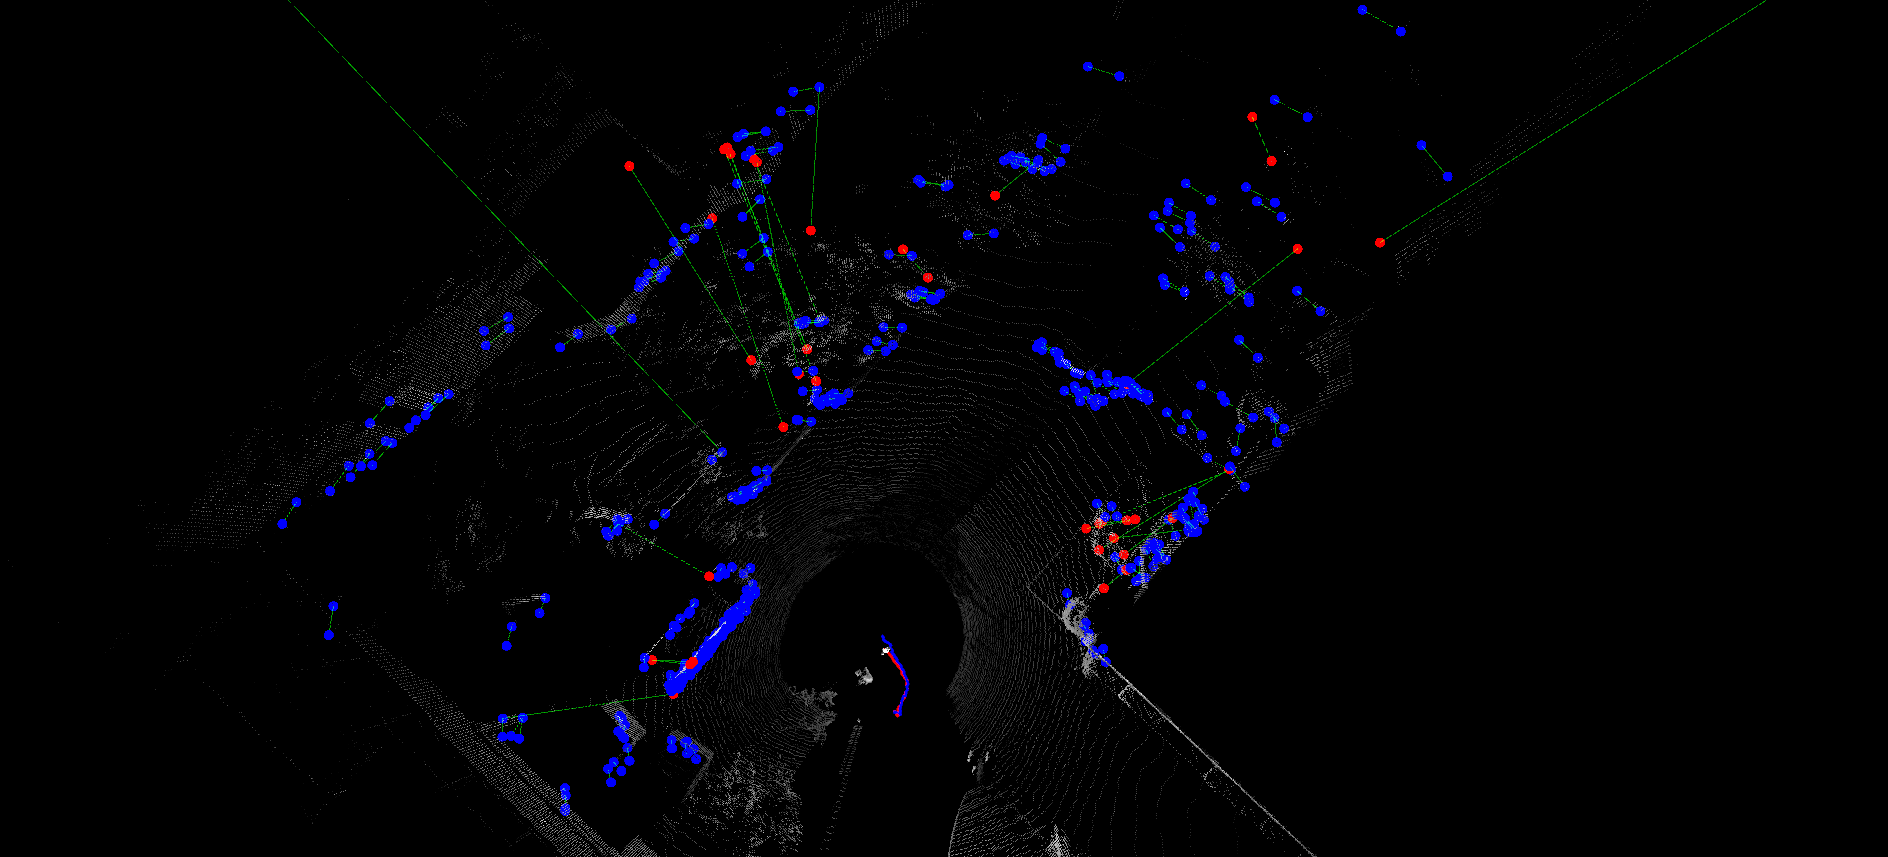
\includegraphics[scale=0.19]{images/matching_+_outlier_rejection/depth_problem_before.png}
            \label{fig:depth_before}
            }\\
        \subfloat[RANSAC + Depth filtered matches]{
        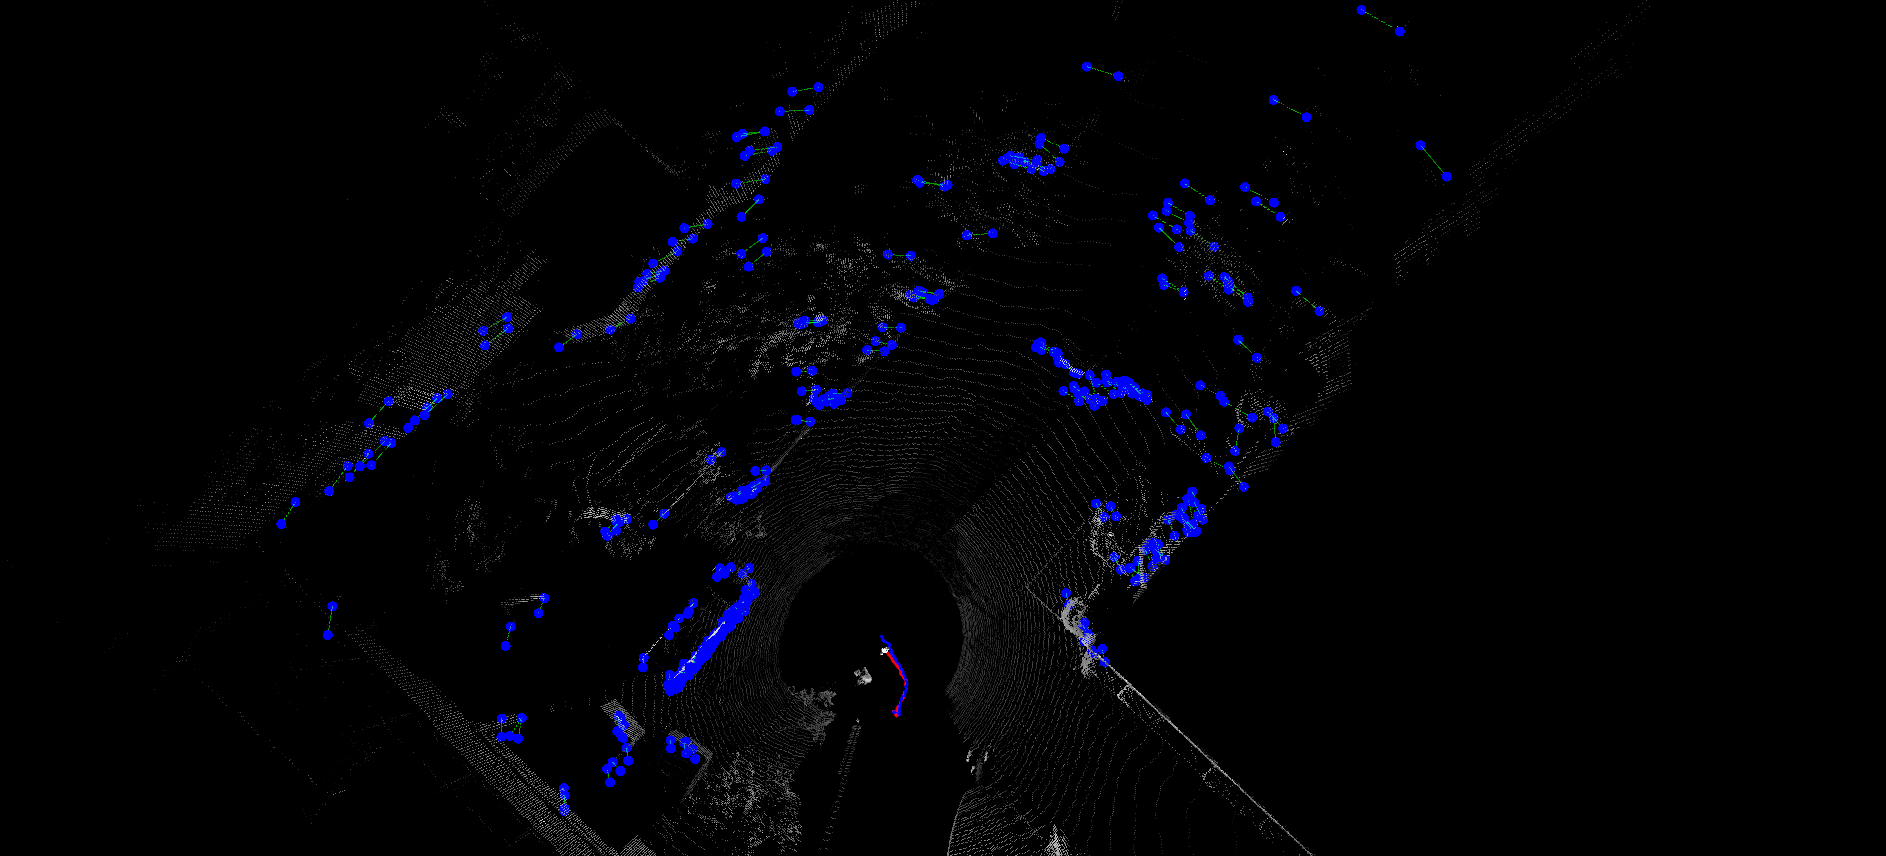
\includegraphics[scale=0.19]{images/matching_+_outlier_rejection/depth_problem_after.png}
            \label{fig:depth_after}
            }
        \caption{Depth problem visualized in Rviz}
        \label{fig:depth_problem}
    \end{figure}

    What we can see on \cref{fig:depth_problem} are correct 3D point correspondences (blue) as well as wrong matches due to depth disparity (red). Note that RANSAC doesn't filter out these red points as they comply with the 2D alignment by chance.

    To resolve this problem the following depth filtering was applied:
}

\clearpage

\section{Depth Filtering}{
    The idea was to filter out all matches with a matching distance in depth direction that surpassed a maximum threshold. To do this I considered two vectors – One from the sensor to a key point (\color{Green}OA\color{black}) and one being the matching vector (\color{orange}AB\color{black}). 

    \begin{figure}[ht]
        \centering
        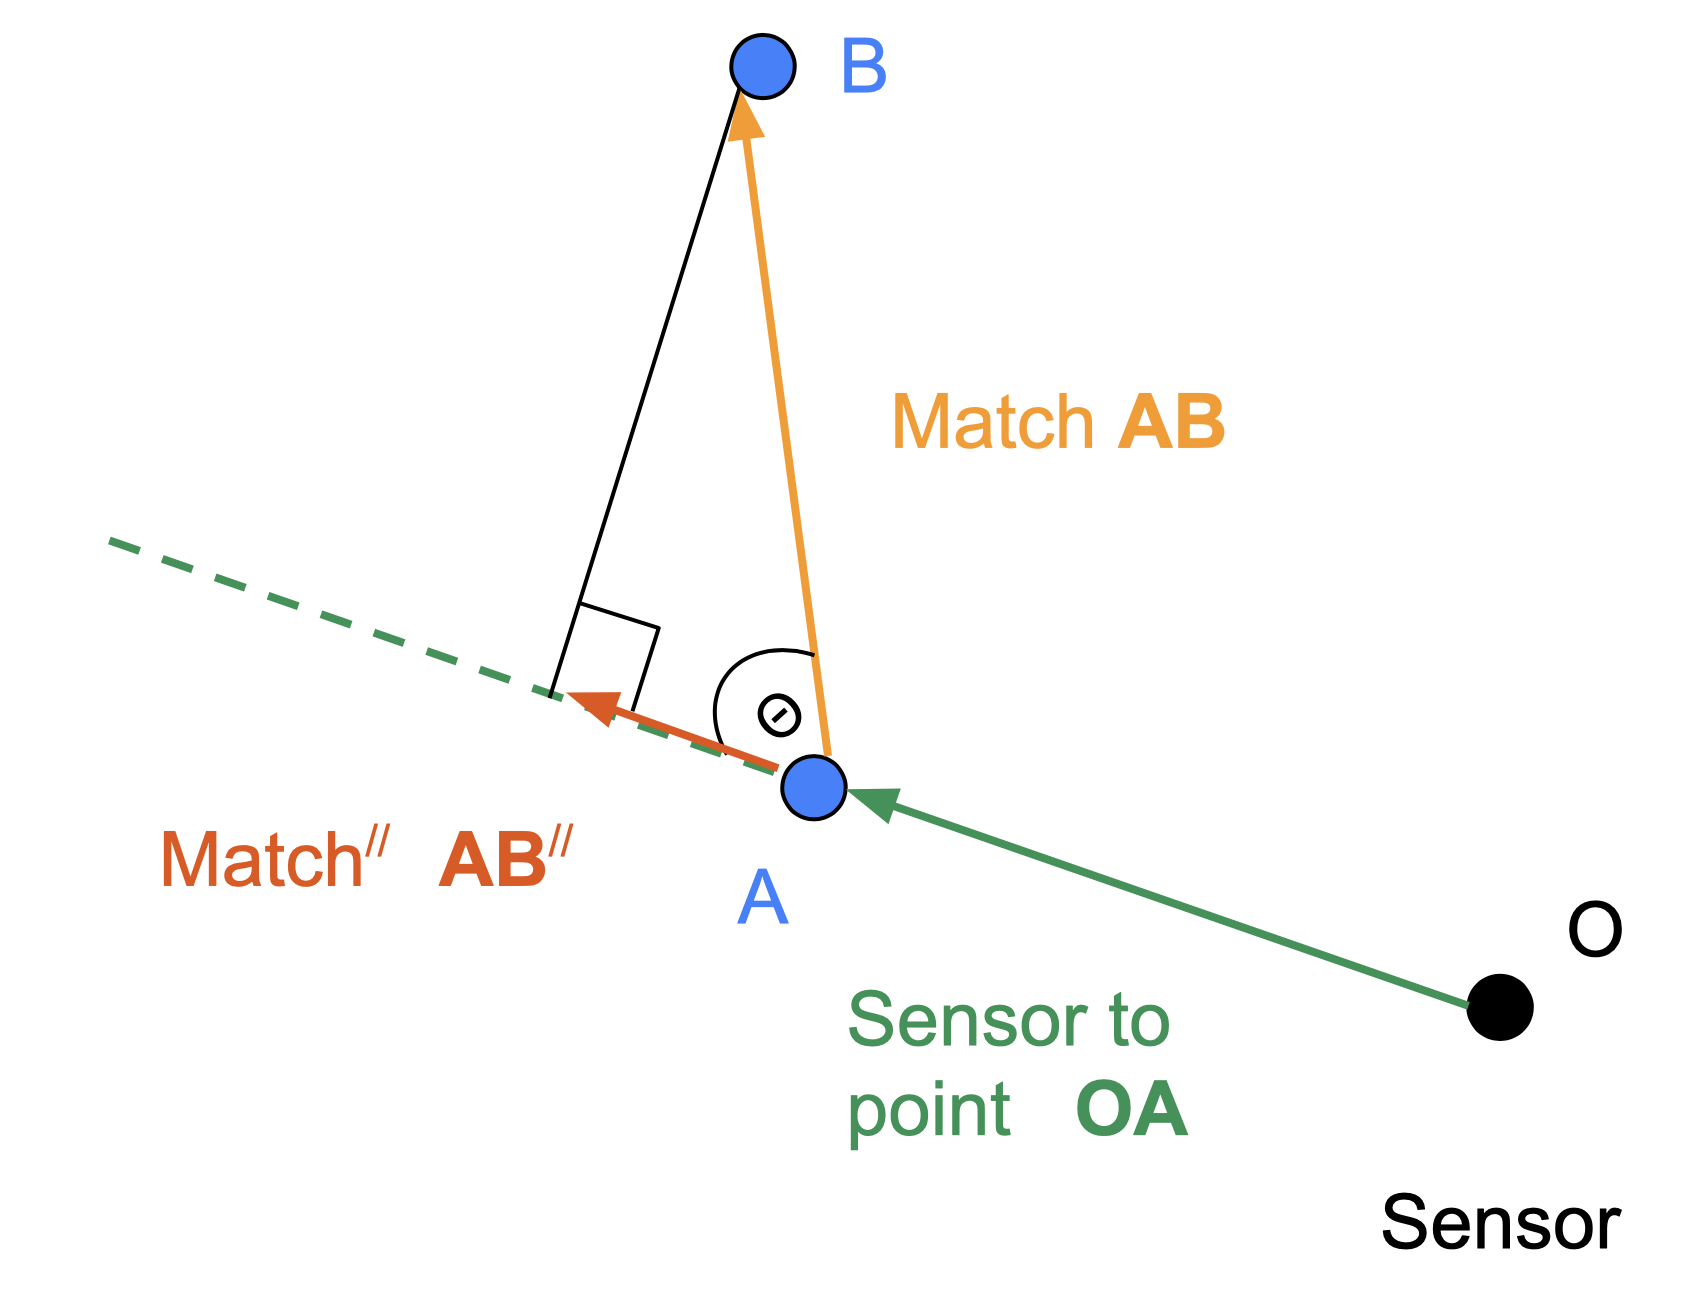
\includegraphics[scale=0.3]{images/matching_+_outlier_rejection/depth_filtering.png}
        \caption{Depth Distance}
        \label{fig:depth_distance}
    \end{figure}

    Then for the filtering I simply considered the projection of AB in depth direction
    
    \begin{center}
        \Large
        $\text{\color{BrickRed}AB\color{black}}^{||} = \frac{\left< \text{\color{Green}OA\color{black}}, \color{orange}AB\color{black}\right>}{||\text{\color{orange}AB\color{black}}||}$
    \end{center}
    and filter out values above a certain threshold. For the handheld dataset I considered at walking speed and 10Hz scanning frequency a distance of 0.3m yielded the best results.

    
}
\clearpage
\section{Feature Method Comparison}{
    After discussing the filtering procedure we can have a look at the match quality comparison. First we compare the different methods used on intensity data:

    \subsection{Visual Comparison}{

        \begin{figure}[htp]
            \centering
            \subfloat[ORB matches]{
                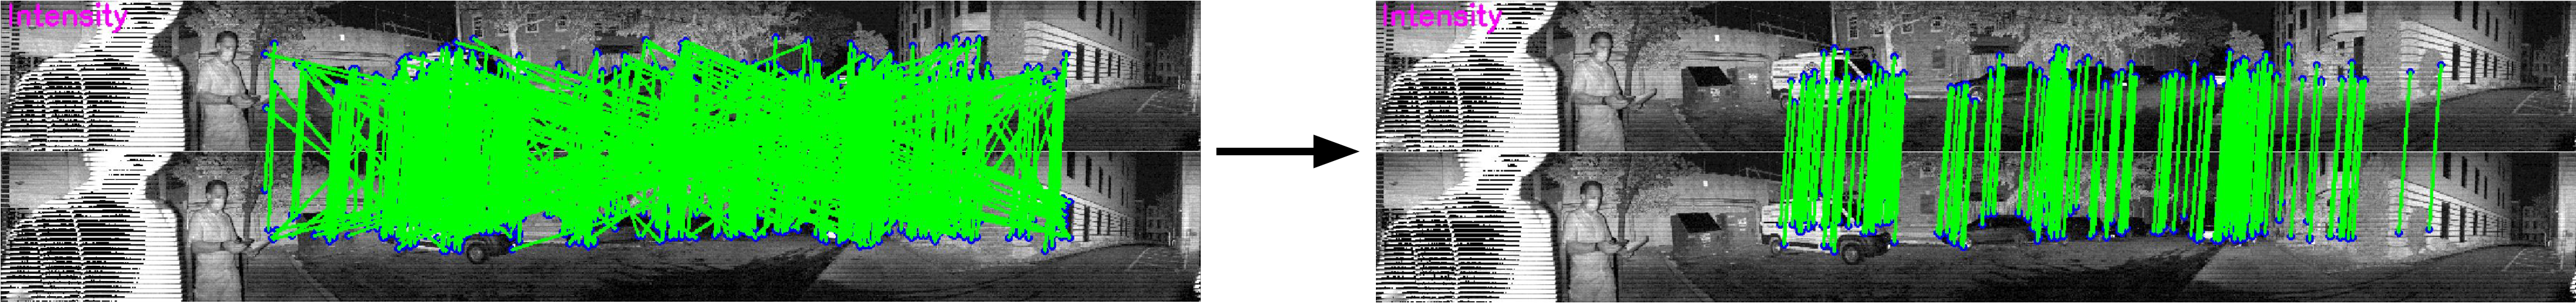
\includegraphics[scale=0.175]{images/matching_+_outlier_rejection/ORB.png}
                \label{fig:ORB_matches}
            }\\
            \subfloat[BRISK matches]{
                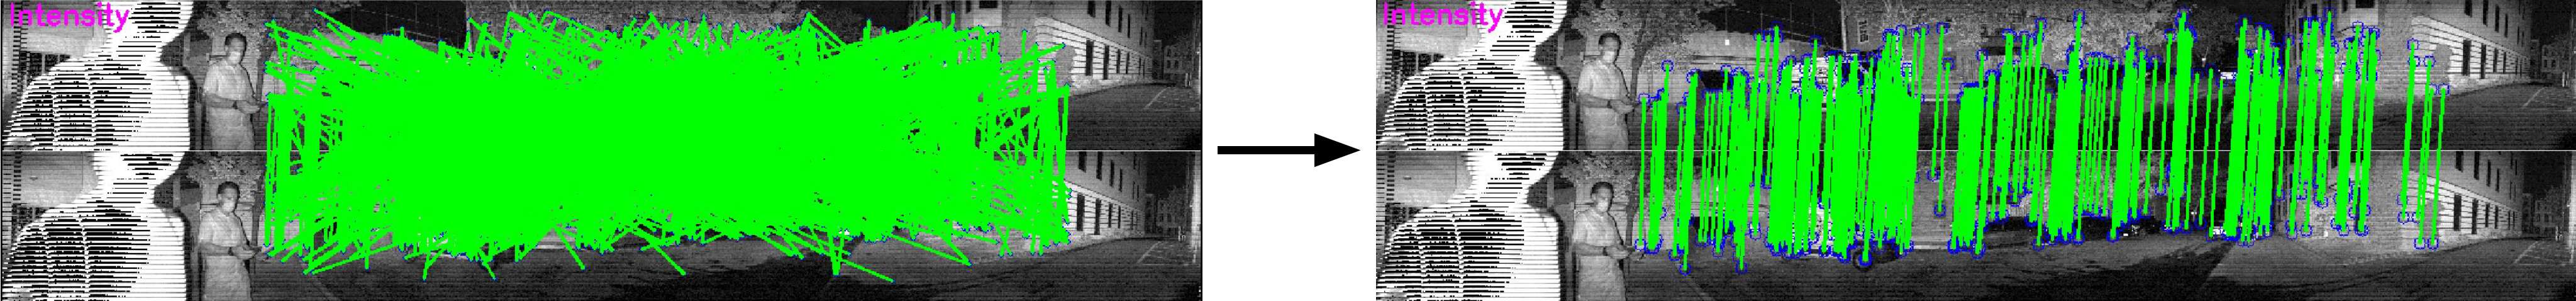
\includegraphics[scale=0.175]{images/matching_+_outlier_rejection/BRISK.png}
                    \label{fig:BRISK_matches}
            }\\
            \subfloat[KLT matches]{
                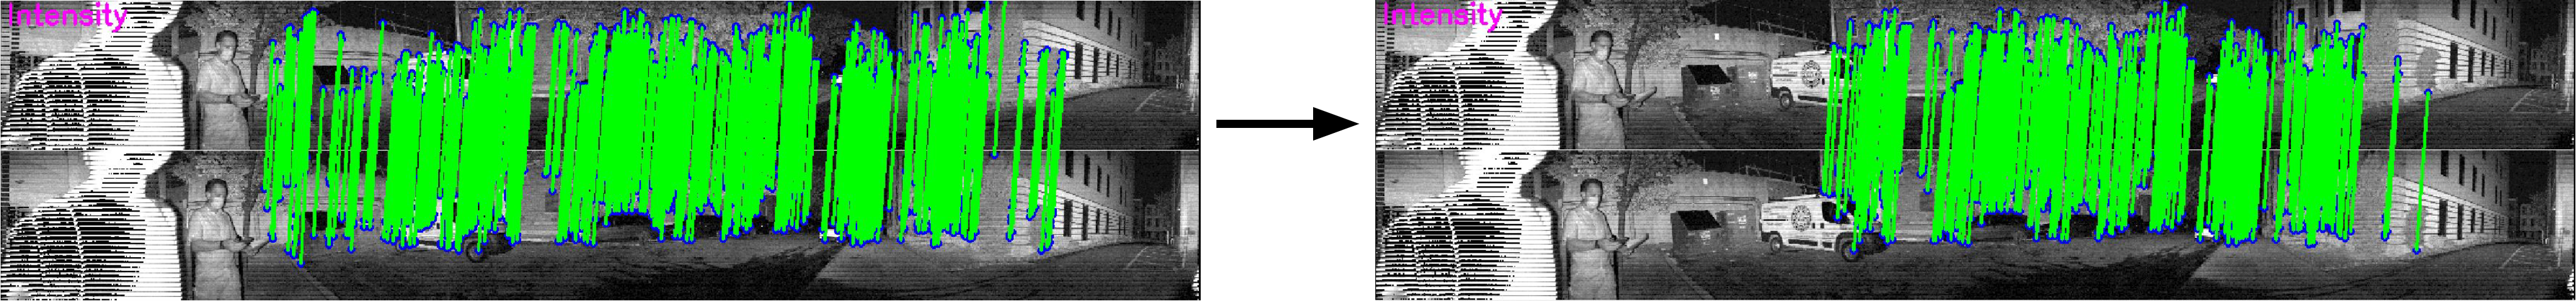
\includegraphics[scale=0.175]{images/matching_+_outlier_rejection/KLT.png}
                    \label{fig:KLT_matches}
            }\\
            \caption{Visual match comparison regarding feature methods}
            \label{fig:match_comparison_descriptors}
        \end{figure}
    
        The arrows indicate the outlier rejection procedure.
    
        As it is only one image the results to be drawn from this are fairly limited. However There seems to be a tendency of BRISK having more initial matches than the other two which complies with the previously found extraction numbers.
    }

    \subsection{Statistical Comparison}{
        As for the extraction comparison I considered the whole dataset and compared the average performance of the different feature techniques:

        \begin{table}[!ht]
            \setlength{\extrarowheight}{10pt}
            \centering
            \begin{tabular}{ccccc}
                & \# Unfiltered Matches & After RANSAC & After Depth & TP Rate [\%]\\[12pt]
                \hline
                ORB & 515 & 190 & 150 & 29.0\\[12pt]
                \hline
                BRISK & 685 & 156 & 123 & 17.9\\[12pt]
                \hline
                KLT & 186 & 151 & 136 & 72.7\\[12pt]
                \hline
            \end{tabular}
            \caption{Matching comparison between methods}
            \label{tab:matching_descriptors}
        \end{table}

        Evaluating the data we see that BRISK creates significantly more matches than ORB while losing more matches to the outlier rejection resulting in a worse TP rate. KLT has fewer correspondences (trackings of points) on average but a much higher TP rate which can be explained by the tracking nature which implicitly doesn't allow radically false  outliers.

    }


    
}

\section{Complementary Data Comparison}{
    \subsection{Visual Comparison}{
        As always the second comparison concerns the different complementary data types.

        Visual comparison using ORB on all source image types:

        \begin{figure}[htp]
            \centering
            \subfloat[Intensity matches]{
                \includegraphics[scale=0.16]{images/matching_+_outlier_rejection/Intensity.png}
                \label{fig:intensity_matches}
            }\\
            \subfloat[Ambient matches]{
                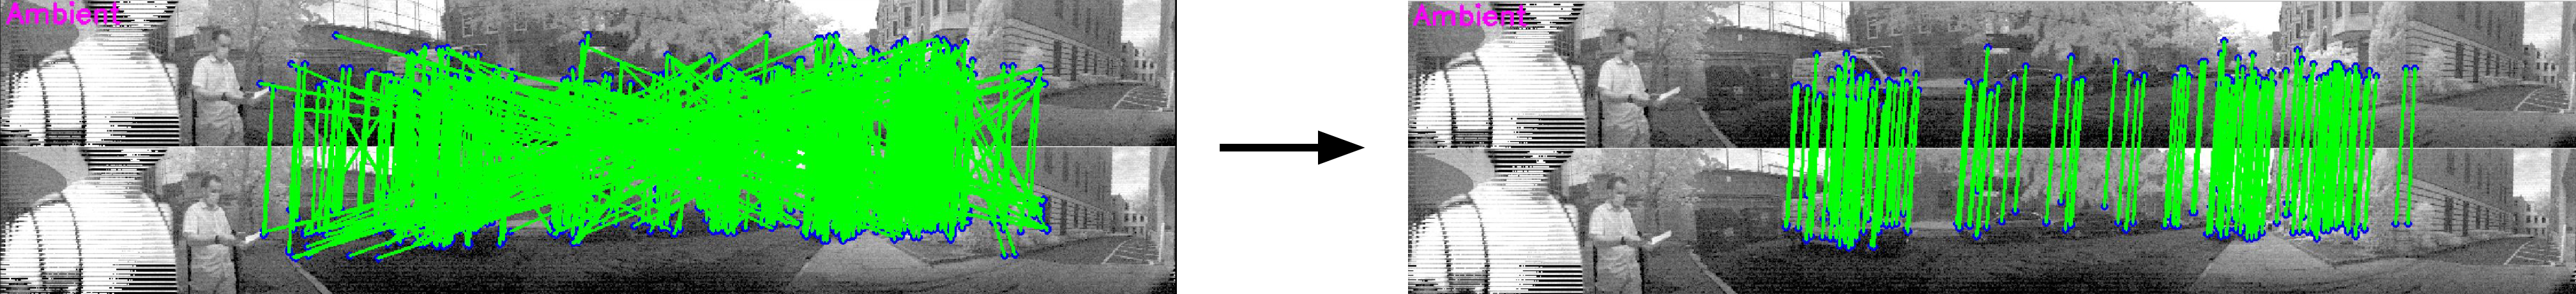
\includegraphics[scale=0.16]{images/matching_+_outlier_rejection/ambient.png}
                    \label{fig:ambient_matches}
            }\\
            \subfloat[Range matches]{
                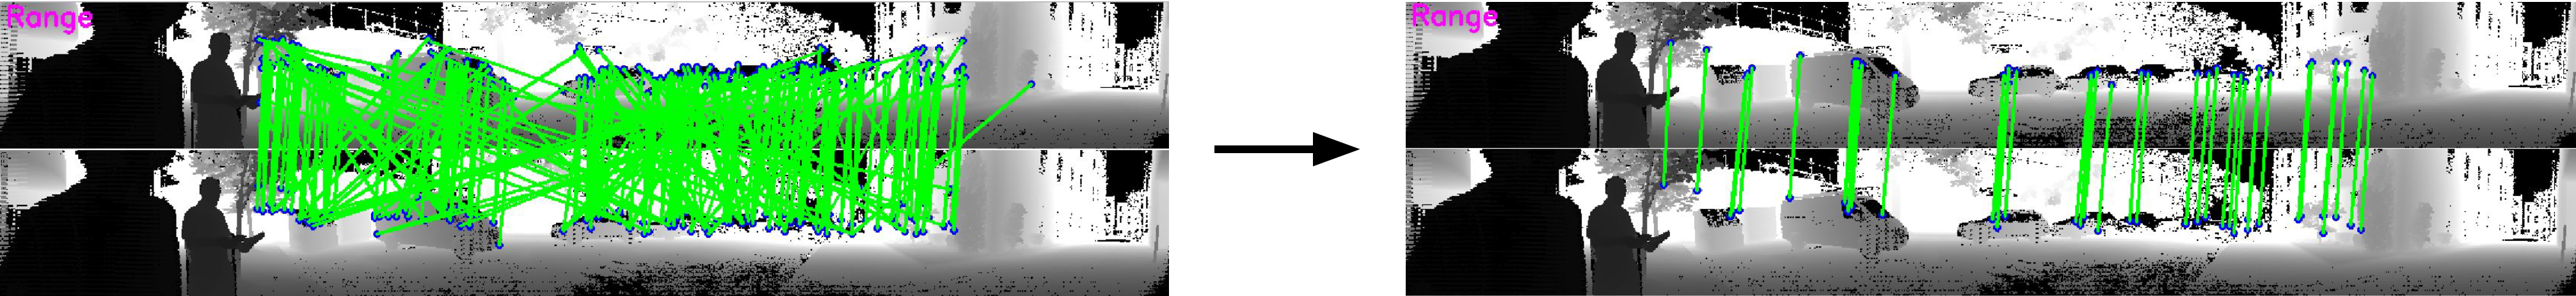
\includegraphics[scale=0.16]{images/matching_+_outlier_rejection/range.png}
                    \label{fig:range_matches}
            }\\
            \caption{Visual match comparison regarding complementary data}
            \label{fig:match_comparison_sources}
        \end{figure}

        We can again see similar performance on intensity and ambient while range has comparatively few initial matches and really few remaining filtered matches in the end.
    }
    \subsection{Statistical Comparison}{
        \begin{table}[!ht]
            \setlength{\extrarowheight}{10pt}
            \centering
            \begin{tabular}{ccccc}
                & \# Intensity Matches & After RANSAC & After Depth & TP Rate [\%]\\[12pt]
                \hline
                Intensity & 515 & 190 & 150 & 29.0\\[12pt]
                \hline
                Ambient & 421 & 164 & 123 & 29.2\\[12pt]
                \hline
                Range & 247 & 61 & 36 & 14.8\\[12pt]
                \hline
            \end{tabular}
            \caption{Matching comparison between data types}
            \label{tab:matching_data}
        \end{table}

        As can be seen ambient and intensity have really similar performance with ambient working with a little fewer matches on average. Range however performs much worse both regarding the amount of matches in general as well as the TP rate.
    }

}